\section{Hierarchical Reinforcement Learning}
When tasks are too complex, it is often easier to decompose it into more manageable sub-tasks. Hierarchical Reinforcement Learning
is a learning paradigm that aims to achieve this using temporal abstraction:

Reasoning on multiple time scales using temporally extended actions (sub-behaviors) that consist of a sequence of primitive actions
and possibly other temporally extended actions.

The following information is derived from \cite{survey_mdpi}.

\subsection{Options Framework}
Here, a popular framework to achieve temporal abstraction in reinforcement learning, the \textit{option framework} \cite{Options}, is described.

\begin{definition}
    An Option is a tuple $\omega = (I, \pi, \beta)$ where
    \begin{itemize}
        \item $I \in \mc{S}$ is the initiation set, which defines the states in which the option can be initiated
        \item $\beta: \mc{S} \rightarrow [0, 1]$ is the termination condition that decides when an option will halt its execution
        \item $\pi: \mc{S} \times \mc{A} \rightarrow [0,1]$ is the intra-option policy.
    \end{itemize}
\end{definition}

A policy-over-options $\pi(\omega|s_t)$ selects an option $\omega \in \Omega$ given a state $s_t$. This additional policy can be useful
to select the best options, when the current state belongs to multiple option initiation sets. It can also be used as an alternative to defining
an initiation set for each option.

The most often used execution model is the call-and-return model. This approach is often also called hierarchical-execution.
In this model a policy-over-options selects an option according to the current state. The agent follows this option until the 
agent triggers the termination condition of the active option.

\begin{figure}[b]
    \centering
    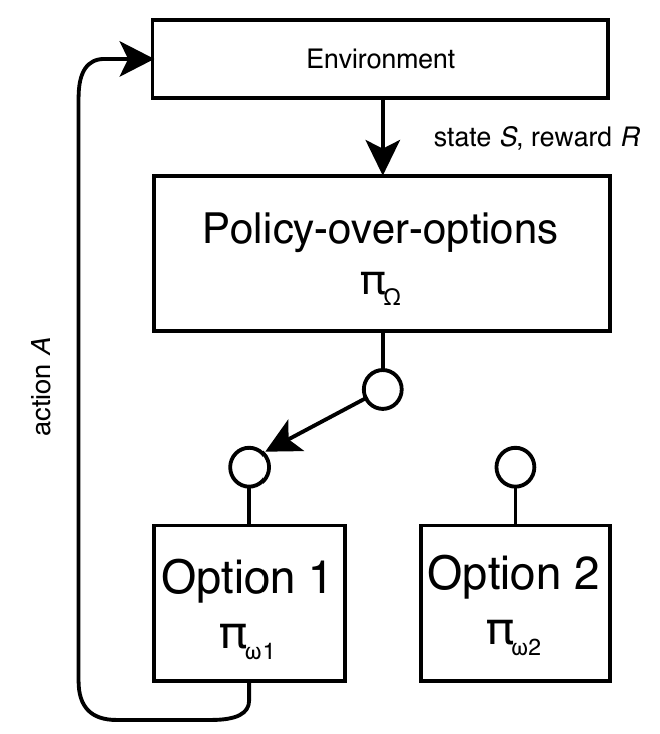
\includegraphics[width=0.3\textwidth]{Images/options_framework.png}
    \caption{Options framework}
    \label{fig:options_framework}
\end{figure}

Motion templates \cite{motion_templates} are options that can be parameterized in order to adapt the behavior of its intra-option policy.
This is often useful in a continuous state-space. A motion template could for example be discovered for throwing a ball. The exhibited
force and angle might be parameters of this template. Learning a single policy for each possible combination of force-angle would be infeasible.

\subsubsection{Option-Critic Framework}

The task of learning options can be decoupled from learning the policy-over-options. The agent can focus first on finding useful temporal
abstractions that simplify the environment. However, this approach of bottom-up learning risks wasting time on learning sub-behaviors which might not be required
in order to solve the problem at hand. Formulating options development and discovery as part of an optimization problem aimed at maximizing the
total future reward is an alternative approach, which allows options and a policy-over-options to be learned end-to-end.

The Option-Critic architecture (OC) \cite{option-critic} is an end-to-end framework capable of discovering and developing options without
using prior knowledge. The actor part in the OC framework consists of multiple intra-options policies. The critic part is capable of assessing discounted
future value of options and actions.

PPOC \cite{PPOC} extends the Option-Critic algorithm for continuous control tasks using PPO \cite{PPO}, a popular on-policy deep reinforcement learning algorithm.

\begin{figure}[H]
    \centering
    \label{fig:options_critic}
    \caption{Option-Critic Architecture.}
    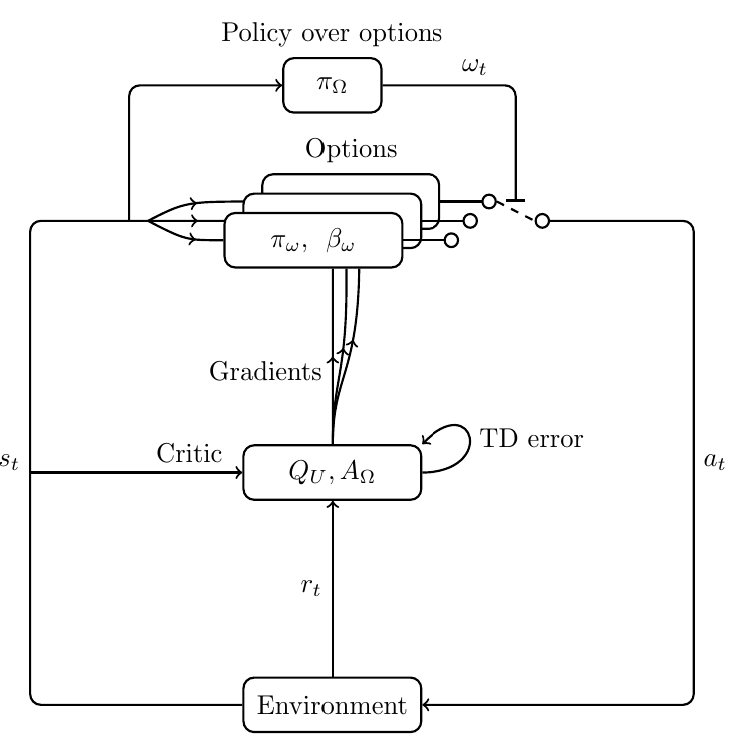
\includegraphics[scale=0.2]{Images/option-critic.png}
\end{figure}

\subsection{Goal-Conditional Framework}

Options are difficult to scale to support numerous sub-behaviors. Training options is inefficient because usually only
one option is trained at the time and no components are shared between them.

Here a different approach is presented; the goal-conditional framework.

The goal-conditional framework models sub-behaviors differently. In order to support a large amount of sub-behaviors,
a goal-vector $z \in Z$ is utilized to express different sub-behaviors.
The goal-vector characterizes the desired sub-behavior activated by a higher level manager to a lower level worker.
The idea is illustrated in Figure \ref{fig:goal-conditional}. This goal-vector can be discrete in order to express
a limited number of abstractions, but it is also possible to use a continuous vector to express an infinite number of possible abstractions.


\begin{figure}
    \centering
    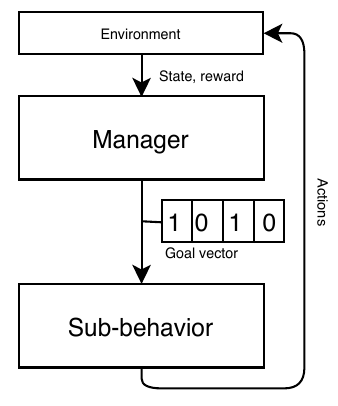
\includegraphics[width=0.3\textwidth]{Images/goal-conditional.png}
    \caption{Goal-Conditional framework.}
    \label{fig:goal-conditional}
\end{figure}

Here are two particular approaches used in the goal-conditional framework:

\begin{itemize}
    \item General Value Function (GVF)
    \item Information Hiding
\end{itemize}

In the \textbf{General Value Function} \cite{Horde} approach different prediction targets are used besides the extrinsic reward signal.
Examples of such targets are: learning how many steps there are
before an episodic control problem terminates; learning the distance before hitting a wall.
Learning different value functions, can be seen as a way to build general knowledge about
how different aspects of the environment can be manipulated. The intuition behind this
idea is that if we know how our environment works, we should be able to achieve
goals in this environment. Different value functions can essentially be utilized as temporal
abstractions, allowing the agent to reason on a higher level of abstraction.
The Horde algorithm \cite{Horde} is capable of learning different targets using independent sub-agents called demons.
Similarly, the Universal Value Function Approximator (UVFA) learns a single value function $V(s, z)$ where the goal-state $z$ is a parameter.
UVFA has also been demonstrated to work in a RL setting, by using Horde.

In the \textbf{Information Hiding} \cite{Feudal_rl} approach no single part of the architecture has access to all available information and different parameters
need to collaborate. While the GVF framework focuses on decomposing the reward function, information hiding focuses on decomposing the state-space.


Algorithms such as HIRO \cite{HIRO} are capable of learning diverse sets of sub-behaviors and their composition, end-to-end, in function
of the extrinsic reward. The HIRO architecture is illustrated in Figure \ref{fig:HIRO}.
In HIRO, the higher level communicates directional subgoals. These subgoals are represented using the state-space and the
lower level is densely rewarded for moving towards this subgoal-state. Other end-to-end algorithms such as FeUdal Networks \cite{FuN}
use a low dimensional latent space to represent sub-behaviors.
The HIRO approach focuses on sample efficiency by supporting off-policy learning. Off-policy corrections are used to
make up for the combinatorial effects introduced by simultaneously learning a lower-level policy and a higher-level policy.
This correction re-labels past experience with a high-level action, in order to maximize the probability of the past lower-level actions.

\begin{figure}
    \centering
    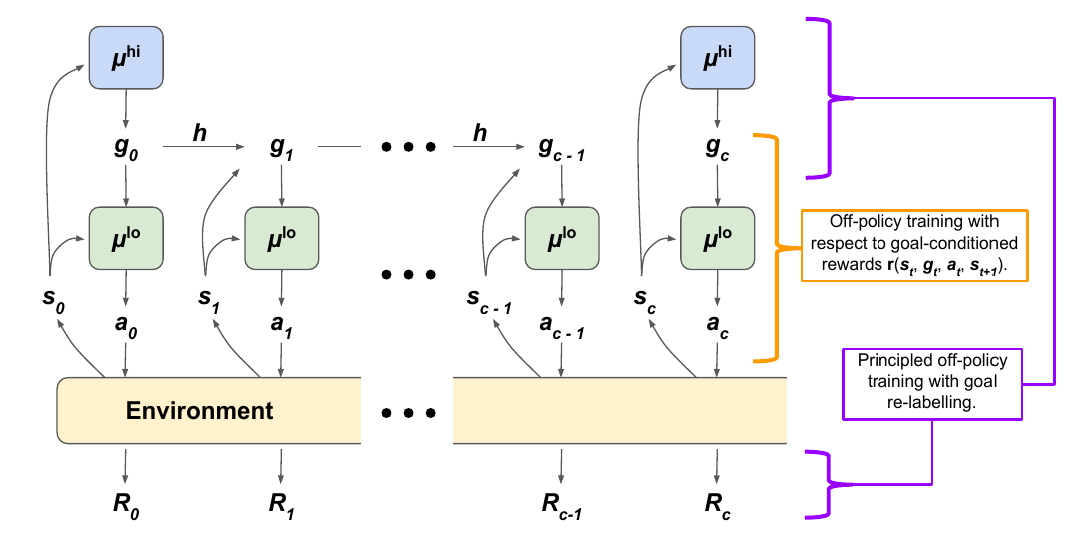
\includegraphics[width=0.8\textwidth]{Images/HIRO.png}
    \caption{HIRO architecture.}
    \label{fig:HIRO}
\end{figure}

